\subsection{Results for $C_{DS}=0.0$}
The following results are for a run with the following input conditions:
\begin{longtable}[c]{A{3.0cm}  A{3.0cm}}
    \caption{Input list for $C_{DS}=0$ test}    \\  \hline
        \textbf{Parameter}      &       \textbf{Value}      \\  \hline
    \endfirsthead
    \caption{Input list for $C_{DS}=0$ test~(continued)}    \\  \hline
        \textbf{Parameter}      &       \textbf{Value}      \\  \hline
    \endhead
        $N$                 &   64      \\
        $t_{final}$         &   100.0   \\
        $C_{DS}$            &   0.0     \\
        $C_{BS}$            &   1.0     \\
\end{longtable}

%\newpage

\begin{figure}[H]
    \begin{subfigure}[H]{0.45\textwidth}
        \includegraphics[height=1.75in]{media/run-cds-00/ke-RHS-CDS-00}
        \caption{$\frac{1}{k} \frac{Dk}{Dt}$}
    \end{subfigure}
    ~
    \begin{subfigure}[H]{0.45\textwidth}
        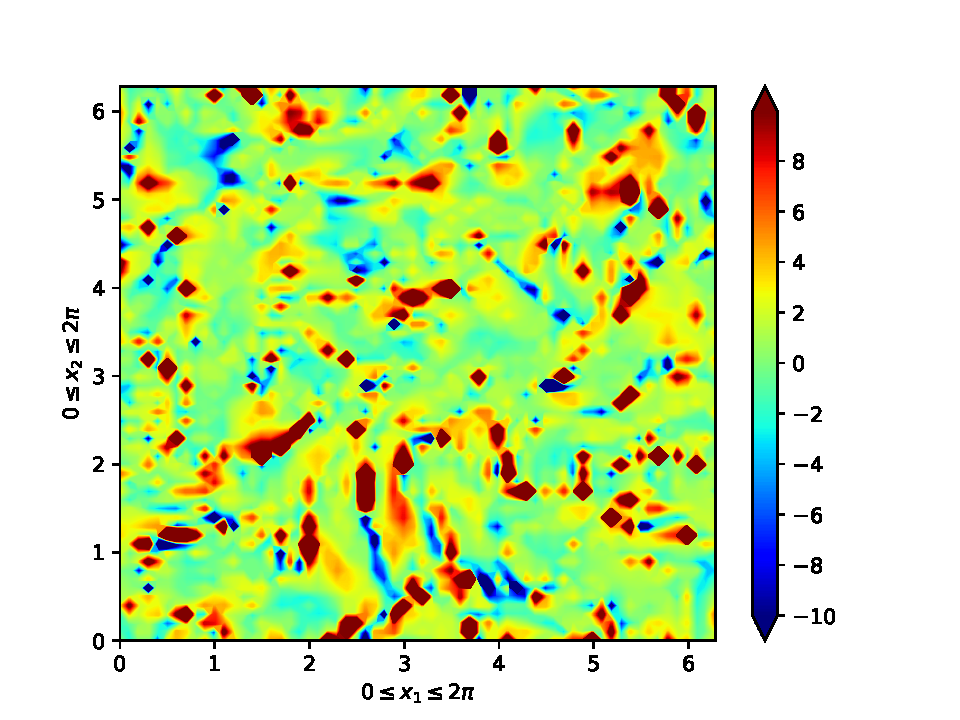
\includegraphics[height=1.75in]{media/run-cds-00/enstrophy-RHS-CDS-00}
        \caption{$\frac{1}{\Omega} \frac{D \Omega}{Dt}$}
    \end{subfigure}
    \newline
    \begin{subfigure}{0.45\textwidth}
        \includegraphics[height=1.75in]{media/run-cds-00/A-enst-CDS-00}
        \caption{$A$}
    \end{subfigure}
    ~
    \begin{subfigure}{0.45\textwidth}
        \includegraphics[height=1.75in]{media/run-cds-00/trans-enst-CDS-00}
        \caption{$\Pi$}
    \end{subfigure}
    \newline
    \begin{subfigure}{0.45\textwidth}
        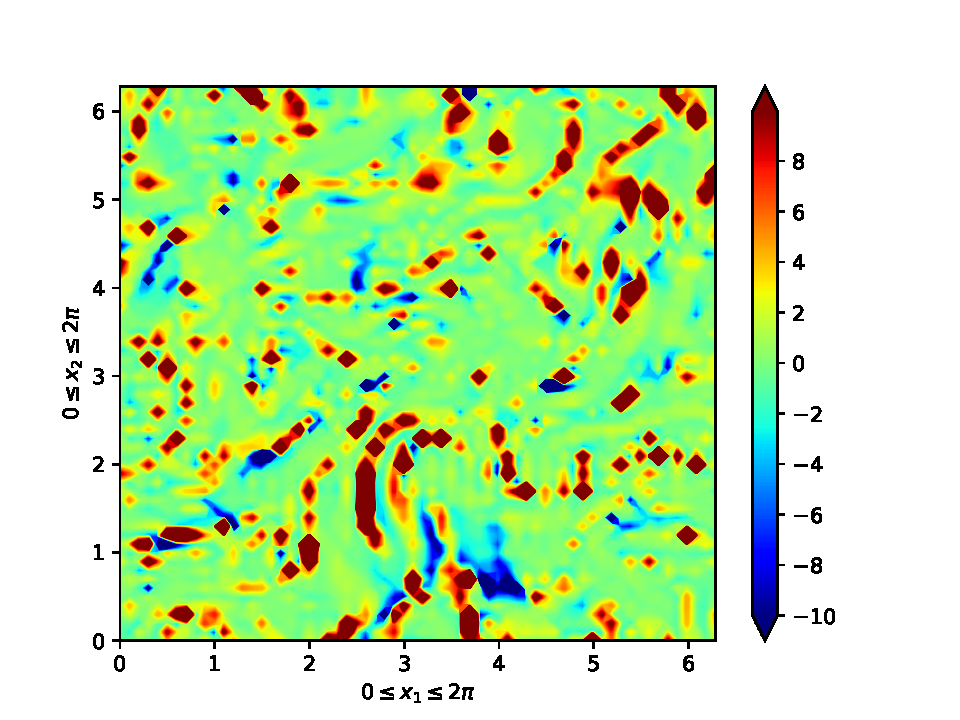
\includegraphics[height=1.75in]{media/run-cds-00/prod-enst-CDS-00}
        \caption{$P$}
    \end{subfigure}
    ~
    \begin{subfigure}{0.45\textwidth}
        \includegraphics[height=1.75in]{media/run-cds-00/B-enst-CDS-00}
        \caption{$B$}
    \end{subfigure}
    \newline
    \begin{subfigure}{0.45\textwidth}
        \includegraphics[height=1.75in]{media/run-cds-00/D-enst-CDS-00}
        \caption{$D$}
    \end{subfigure}
\end{figure}
%\newpage
\subsection{Results for $C_{DS}=0.65$}
\begin{figure}[H]
    \begin{subfigure}[H]{0.45\textwidth}
        \includegraphics[height=1.75in]{media/run-cds-65/ke-RHS-CDS-65}
        \caption{$\frac{1}{k} \frac{Dk}{Dt}$}
    \end{subfigure}
    ~
    \begin{subfigure}[H]{0.45\textwidth}
        \includegraphics[height=1.75in]{media/run-cds-65/enstrophy-RHS-CDS-65}
        \caption{$\frac{1}{\Omega} \frac{D \Omega}{Dt}$}
    \end{subfigure}
    \newline
    \begin{subfigure}{0.45\textwidth}
        \includegraphics[height=1.75in]{media/run-cds-65/A-enst-CDS-65}
        \caption{$A$}
    \end{subfigure}
    ~
    \begin{subfigure}{0.45\textwidth}
        \includegraphics[height=1.75in]{media/run-cds-65/trans-enst-CDS-65}
        \caption{$\Pi$}
    \end{subfigure}
    \newline
    \begin{subfigure}{0.45\textwidth}
        \includegraphics[height=1.75in]{media/run-cds-65/prod-enst-CDS-65}
        \caption{$P$}
    \end{subfigure}
    ~
    \begin{subfigure}{0.45\textwidth}
        \includegraphics[height=1.75in]{media/run-cds-65/B-enst-CDS-65}
        \caption{$B$}
    \end{subfigure}
    \newline
    \begin{subfigure}{0.45\textwidth}
        \includegraphics[height=1.75in]{media/run-cds-65/D-enst-CDS-65}
        \caption{$D$}
    \end{subfigure}
\end{figure}
